
%%%%%%%%%%%%%%%%%%%%%%
%                                                                 %
% COMMERCIAL SOFTWARES REVIEW  %
%                                                                 %
%%%%%%%%%%%%%%%%%%%%%%

%COMMERCIAL SOFTWARES REVIEW
\chapter{Review of Available Geochemical Modeling Software}
\label{chapter:review}
The first geochemical models date back to the 70’s \cite{Westall:76},~\cite{Wolery:1979}. 
Since then, these models are used to solve complex geochemical problems, such as speciation; determination of minerals' saturation indexes; mixing of different waters; calculation of stoichiometric reactions; interaction between solids, fluids and gaseous phases; calculation of equilibrium/kinetic controlled reactions; reactive transport; and mass-law calculations.

The quality of model results depend on the methods used, and the thermodynamic data and theoretical concepts applied. Therefore, it is crucial to verify the results and it is clear that there will be some differences among the results obtained from different software. Among the enormous variety of software available, some of them are developed for batch-type simulations only, while others have transport capabilities. Several of them do not incorporate graphical interfaces and are written in \emph{FORTRAN}, while newer distributions are mainly written in C/C++ and, due to proprietary reasons, code is not distributed with the software. It is important to mention that, even in those who provide an integrated graphical user interface (\emph{GUI}), it is often very tedious and time-consuming to generate input files for simulations.


For developing SHPECK, we critically analysed the software packages that provide speciation modeling: \emph{EQ3/6}, \emph{PHREEQC}, \emph{MINTEQ} and \emph{SOLMINEQ}. We had given special attention to the geochemical modeling approaches and the computer-science related aspects of them, providing the comparison when the information is available. We also summarize the main characteristics and content of the Lawrence Livermore National Laboratory (\emph{LLNL}) Thermodynamic Dataset, since it contains parameters of minerals and reactions used by many modeling software.


%GEOCHEMICAL SPECIATION MODELING CODES
%\section{Geochemical Speciation Modeling Software}

%EQ3/6
\section{\emph{EQ3/6}}
EQ3/6 consists of two programs: EQ3 is a pure speciation code, whose results EQ6 subsequently process. It is a software package for geochemical modeling of aqueous systems written in FORTRAN77. 
EQ3/6 includes a speciation-solubility solver, which is useful for analyzing groundwater chemistry data, calculating solubility limits and determining whether certain reactions are in states of partial equilibrium or disequilibrium. It also offers a reaction path calculation that models water/rock interaction or fluid mixture. 
EQ3/6 supports several thermodynamic data files (these data files contain support for \emph{Davies}, \emph{B-dot}, \emph{Debye-Huckel} equations, as well as support data for standard state and activity coefficient-related). 
It is developed to run under UNIX, and the full package distribution is not free (it requires a license). The whole work related to EQ3/6 is described in three reports: \cite{Wolery:1979}, \cite{Wolery:1990} and \cite{Wolery:1992}.

\subsection{Input/Output Options}
The \emph{datafilekey} and \emph{inputfile} are files given to the program as arguments and they must be mutually consistent with the options and methods. For example, if they have different methods for calculating the activity coefficient there will be problems, and the results will be erroneous. In the similar manner, the \emph{inputfile} must be using chemical data (for example, elements, species and compounds) that is known by the \emph{datafilekey}.

Inside each file, there are a series of \emph{blocks} that are combined to support the geochemical speciation. They are presented below:
\begin{itemize}
\item \emph{Datafilekey}: Title; Miscellaneous parameters (temperature limit, activity coefficient parameters, pressure); chemical elements block; aqueous species block; pure minerals block; pure non-aqueous liquids block; gas species blocks; solid solutions blocks; references blocks.
\item \emph{Inputfile}: Title; Special basis switches; temperature; pressure option; density; total dissolved salts (TDS) option; electrical balancing option; redox option; basis species constraints; ion exchanger creation flag; ion exchanger compositions; solid solutions compositions; alter/suppression options; iopt options; iopg options; iopr options; iodb options; numerical parameters; ordinary basis switches; saturation flag tolerance; aqueous phase scale factor.
\end{itemize}

EQ3/6 package produces different outputs depending on the version of software used. We will exemplify the output files in general by using the \emph{EQ3NR} and \emph{EQ6} output formats. 
\begin{itemize}
\item \emph{EQ3NR}: Two output files are generated: a \emph{pickup} file and the normal output file. The \emph{pickup} file can be used as input to \emph{EQ6} software. The normal output file consists of six blocks: header section; input file echo; recap of input data; iterative calculations; principal results; and finally the end of EQ3NR run
\item \emph{EQ6}: This program generates three output files: a \emph{tab} output file, a \emph{pickup} output file and the normal output file. The \emph{tab} file contains information that can be used to plot output results. The \emph{pickup} file is the input to \emph{EQ6}. The normal output file of \emph{EQ6} is similar to the \emph{EQ3NR}'s output file.
\end{itemize}

A small excerpt of an \emph{EQ6} output file is shown in Code~\ref{eq3:output}. We can observe that this part of the output file specifies the components of the current problem with internal ID's for each component, specie, phase and so on.

\begin{minipage}[c]{0.92\textwidth}
\begin{lstlisting}[frame=single, caption=Excerpt of \emph{EQ6} output file, label=eq3:output]
...
 Entity Date Base Dimension Current Problem
 Chemical Elements 81 81 6
 Basis Species 201 259 7
 Phases 1135 1159 29
 Species 3031 3523 0
 Aqueous Species 1769 1769 22
 Pure Minerals 1120 1120 26
 Pure Liquids 1 3 1
 Gas Species 93 93 2
 Solid Soutions 12 12 0
...
\end{lstlisting}
\end{minipage}

\subsection{User Interaction}
In \emph{EQ3/6} the command prompt is used for all the user interaction. There are several functions inside \emph{EQ3/6}; the appropriate command will trigger each one of them. From the existing software, there are \emph{EQ3NR}, \emph{EQ6} and \emph{EQPT}, just to name a few. The user must enter the command from the keyboard and must use this "command prompt". By pressing "CTRL+C" at any time the execution stops, literally "breaking" the process. For example, EQ3 is run by commands of the form shown in code ~\ref{eq3:run}.

\begin{lstlisting}[frame=single, caption=Running EQ3 in \emph{EQ3/6} package, label=eq3:run]
>runeq3 datafilekey inputfile(s)
\end{lstlisting}

In this command, \emph{datafilekey} and \emph{inputfile} are arguments, being the former a three-character identification associated to which database should be used, while the latter is specifically the name of the input file, which can be more than one. Depending on which program from the package the user is using, it generates two or more output files (always in the \emph{ASCII} format).
As mentioned, the input file is entered in the program as an argument. Any regular text editor is sufficient to create or modify an input file (although it is not recommended that the user create an input file from scratch). There are several pre-existing input templates available and, if none of them matches the need of the user, \emph{EQ3/6} recommends that the user generate a new one by copying existing blocks from any provided template.

The input files can contain instructions and parameters that try to recreate known user interactions method as shown in Code ~\ref{eq3:menu}.

\begin{minipage}[c]{0.92\textwidth}
\begin{lstlisting}[frame=single, caption=Menu Option inside \emph{EQ3/6} input files that mimics a "radio button", label=eq3:menu]
iopr(4) - Print a Table of Aqueous Species Concentrations, Activities, etc.: 
 [ ] (-3) Omit species with molalities < 1.e-8 
 [ ] (-2) Omit species with molalities < 1.e-12 
 [ ] (-1) Omit species with molalities < 1.e-20 
 [x] ( 0) Omit species with molalities < 1.e-100 
 [ ] ( 1) Include all species 
\end{lstlisting}
\end{minipage}

% VEJA E-MAIL SOBRE ESSE TEXT FILE QUE É DATABASE ABAIXO 
% Reformatei todo o paragrafo, tirando o foco do especifico problema de text/binary, mas salientando que o uso desse tipo de arquivo acaba gerando desperdicio de memoria que é importante... a ideia permanece a mesma, mas com outro appraoch..deixando bem claro em qualquer linguagem, eu imagino..
\subsection{File Formats}
All the files discussed above are \emph{ASCII} text files and, therefore, any regular text editor can be used to edit or build them. When the text file contains thermodynamic information needed by the program, the whole group of information is copied to the memory and, only after that, the software will be able to fetch information and continue the simulation's processing and natural flow. In memory, the storage of this information is not always optimized, specially because \emph{ASCII} files are, in general, also not very well organized. Waste of memory here and there are expected and usual in this kind of text and memory management - scale this to a large amount of \emph{ASCII} information - like in geochemical modeling systems - and it is easy to understand the risk that comes together with \emph{ASCII} text files. 

% TENHO DUVIDA - ACHO QUE NÃO PRECISA ESSA SEÇÃO DE INSTALAÇÃO
\subsection{Software Environment and Installation Procedures}
The \emph{EQ3/6} package runs on Windows (95 and upper versions) and was developed in FORTRAN77. The support for UNIX computers has been discontinued.  It has been developed and run at \emph{Lawrence Livermore National Laboratory} on an \emph{Alliant FX/80} and \emph{Sun SPARCstations}.

The installation of \emph{EQ3/6} is explained in details in ~\cite{Wolery:1992}, and these details will be suppressed here for simplicity. However, it is interesting to mention that the whole installation process requires some level of experience with command prompt and \emph{DOS}.



%PHREEQC
\section{\emph{PHREEQC}}
\emph{PHREEQC} stands for \emph{PH} \emph{RE}dox \emph{EQ}uilibrium in \emph{C} language, and is a widely used geochemical modeling software available from the USGS. Details can be found in \cite{Parkhurst:95}. It is available for download in versions for Windows and UNIX. 

It was designed to perform a wide variety of low-temperature aqueous geochemical calculations based on an ion-association aqueous model, and has capabilities to:
\begin{itemize}
\item speciation and Saturation Index calculations;
\item batch reaction and one-dimensional (1D) transport calculations involving reversible reactions (including aqueous, minerals, gas, solid-solution, surface-complexation, and ion-exchange equilibrium) and irreversible reactions (including specified mole transfer of reactants, kinetically controlled reactions, mixing of solutions and temperature changes);
\item inverse modeling, which finds sets of mineral and gas mole transfers that takes into account differences in composition between waters.
\end{itemize}

\subsection{Input/Output Options}
The input data for \emph{PHREEQC} is arranged by \emph{keyword data blocks}. Each block is organized with a keyword in the first line, followed by lines containing data related to the keyword. Keywords and their respective contexts are read from the database at the beginning of the run to define all the necessary parameters. After this database reading procedure, it continues reading the input file until it reaches the \emph{END} keyword. As the input file is being read, the program starts putting the pieces together to perform the necessary calculations. An example of a \emph{keyword data block} is shown in Code~\ref{phreeqc:keyword}. Among the possible keywords available in \emph{PHREEQC} are EQUILIBRIUM PHASES, EXCHANGE, GAS PHASE, INVERSE MODELING, PHASES, REACTION, PRINT, SAVE, SOLUTION SPECIES, etc. Each one of these keywords contains specific arguments and parameters to be used. Certain keywords require some other specific keywords, and if something is missing from the input file, the results will be inconclusive. So, building an input file is usually a quite difficult and time-consuming task. 

\begin{minipage}[c]{0.92\textwidth}
\begin{lstlisting}[frame=single, caption=\emph{PHREEQC} keyword data block example, label=phreeqc:keyword]
EQUILIBRIUM_PHASES
Chalcedony  0.0     0.0
CO2(g)      -3.5    1.0
Gibbsite(c) 0.0     KAlSiO8  1.0
Calcite     1.0     Gypsum   1.0
pH_Fix      -5.0    HCl      10.0
\end{lstlisting}
\end{minipage}

The output file contains the result of the simulation defined in the input file; it is also divided into \emph{keyword blocks}. Among those blocks are solution composition, description of the solution, redox couples, distribution of species (as can be seen in Code~\ref{phreeqc:output}), and saturation indices.

\begin{minipage}[c]{0.92\textwidth}
\begin{lstlisting}[frame=single, caption=\emph{PHREEQC}'s excerpt from the output file, label=phreeqc:output]
...
----------------------------Distribution of species----------------------------
 
                                               Log       Log       Log    mole V
   Species          Molality    Activity  Molality  Activity     Gamma   cm3/mol
 
   OH-            2.705e-006  1.647e-006    -5.568    -5.783    -0.215     -2.63
   H+             7.983e-009  6.026e-009    -8.098    -8.220    -0.122      0.00
   H2O            5.551e+001  9.806e-001     1.744    -0.009     0.000     18.07
C(4)         2.257e-003
   HCO3-          1.238e-003  8.359e-004    -2.907    -3.078    -0.170     27.87
   NaHCO3         6.168e-004  7.205e-004    -3.210    -3.142     0.067     19.41
   MgHCO3+        2.136e-004  1.343e-004    -3.670    -3.872    -0.201      5.82
   MgCO3          7.301e-005  8.527e-005    -4.137    -4.069     0.067    -17.09
   CaHCO3+        3.717e-005  2.572e-005    -4.430    -4.590    -0.160      9.96
   CO3-2          3.128e-005  6.506e-006    -4.505    -5.187    -0.682     -0.34
   CaCO3          2.256e-005  2.636e-005    -4.647    -4.579     0.067    -14.60
   NaCO3-         1.477e-005  9.972e-006    -4.831    -5.001    -0.170      1.77
...
\end{lstlisting}
\end{minipage}

\subsection{User Interaction}
\emph{PHREEQC}'s distribution differs drastically according to the environment (\emph{Windows} or \emph{UNIX}). By this reason, the analysis of user interaction features will be reported separately.

\begin{itemize}
\item \emph{PHREEQC} for Windows: Due to the need of a geochemical modeling software and the lack of interface for \emph{PHREEQC} in the first versions of the software, many efforts were made to create an interface to \emph{PHREEQC}. The program \emph{PhreeqcI} is a graphical user interface to \emph{PHREEQC} that provides data entry screens for the keyword data blocks with a description of each input data item. It organizes the input file by using some \emph{project tree} which facilitates viewing, selecting, editing and running the \emph{PHREEQC} simulations. It is critical to mention that \emph{PhreeqcI} does not implement all the keyword blocks. Subsequently, \emph{PHREEQC} version 2 with a graphical interface was launched, and the interface was extended to version 3. This graphical interface was named \emph{PfW} (\emph{Phreeqc for Windows}), but it has not been updated since 2011 (see Figure~\ref{fig:phreeqc-pfw}). The last effort in this sense was the development of an adaptation of the popular general-purpose text editor \emph{Notepad++}. This modification comes with the following capabilities: syntax highlighting; autocompletion of keywords and identifiers; tips; colored numbers; parenthesis matching; commenting and uncommenting multiple lines at once; column editor; few shortcuts; and file recognition (see Figure~\ref{fig:phreeqc-notepad++}). When running \emph{PHREEQC} from the \emph{Notepad++} adaptation, the command prompt is called and the simulation is executed, as in Figure~\ref{fig:phreeqc-notepad++2}. There are some options and shortcuts available from the \emph{Notepad++}'s interface, which is shown in detail in Figure~\ref{fig:phreeqc-notepad++3}.
\item \emph{PHREEQC} for \emph{UNIX}: Under \emph{UNIX}'s distribution, \emph{PHREEQC} runs from the command prompt. It can be launched by using the command shown in Code~\ref{phreeqc:run}
\begin{lstlisting}[frame=single, caption=Command to run UNIX's \emph{PHREEQC}, label=phreeqc:run]
phreeqc input output database screen_output
\end{lstlisting}
The \emph{"input"} file contains the description of the simulation, the \emph{"output"} file stores the result of the simulation, \emph{"database"} specifies which database should be used, and finally the \emph{"screen\_output"} stores the information that will be shown on screen. If the user does not specify the names of \emph{"output"}, \emph{"database"} or \emph{"screen\_output"} the geochemical modeling software will choose default values.
\end{itemize}

\begin{figure}[ht!]
\centering
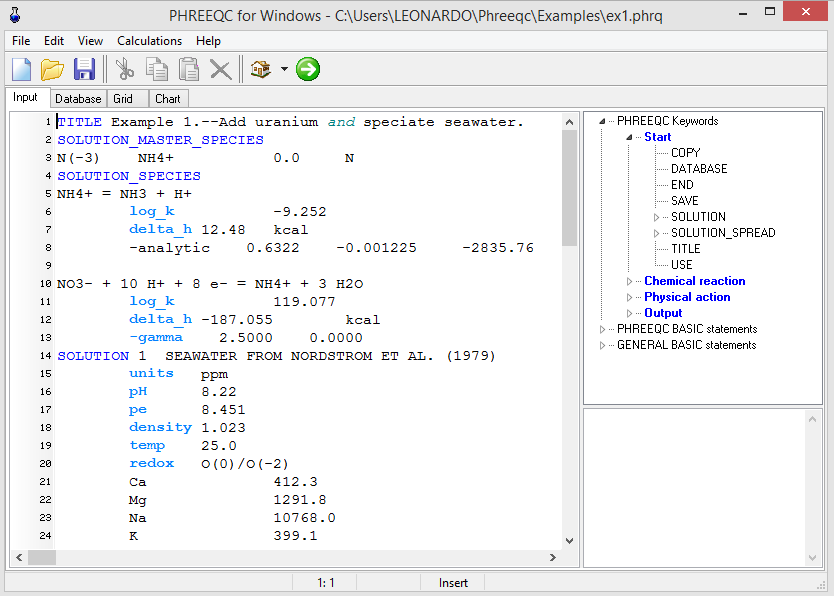
\includegraphics[width=100mm]{figures/pfw.png}
\caption{User interface of the PHREEQC for Windows (\emph{PfW})}
\label{fig:phreeqc-pfw}
\end{figure}

\begin{figure}[ht!]
\centering
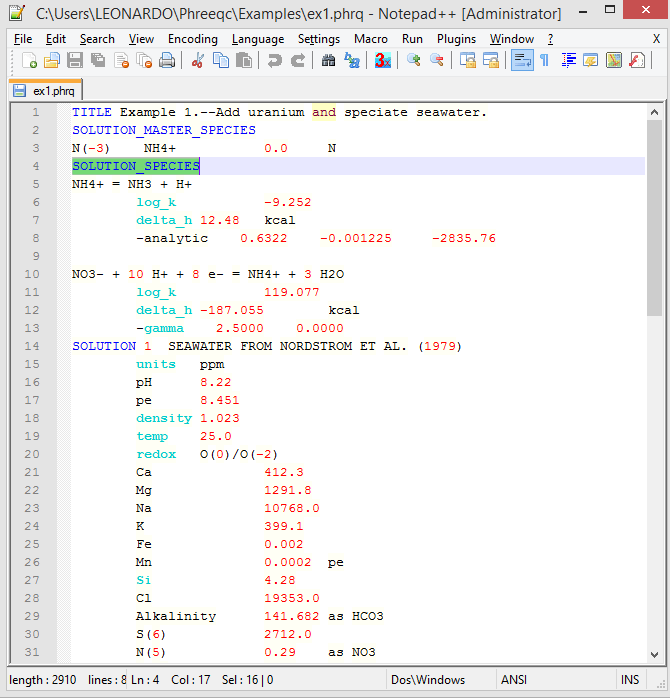
\includegraphics[width=100mm]{figures/notepad++Phreeqc.png}
\caption{Example of the PHREEQC Notepad++ plugin}
\label{fig:phreeqc-notepad++}
\end{figure}

\begin{figure}[ht!]
\centering
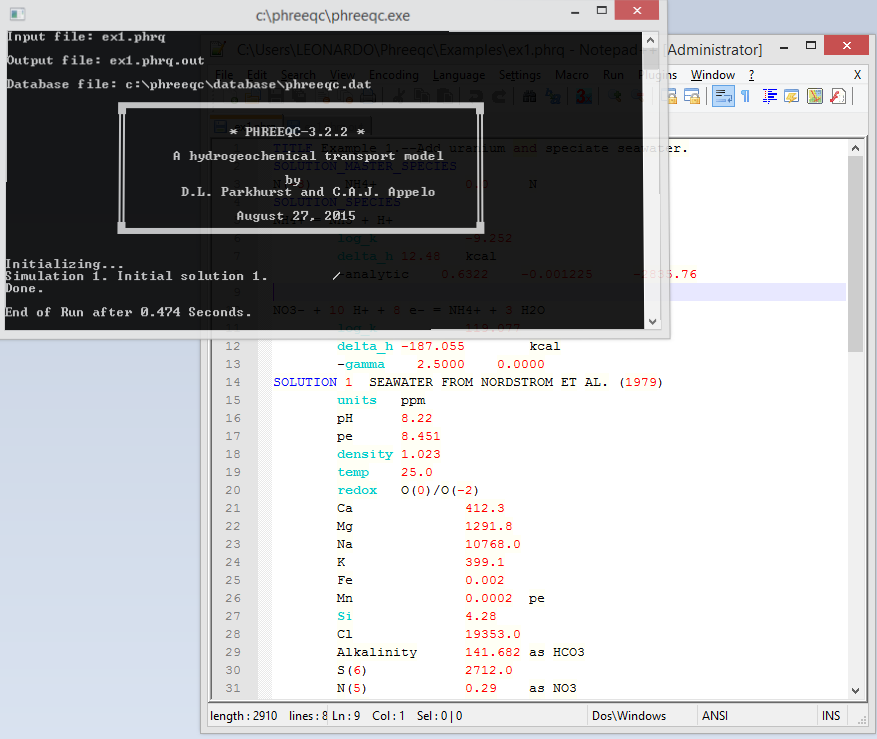
\includegraphics[width=100mm]{figures/notepad++PhreeqcProcess.png}
\caption{PHREEQC software called from the Notepad++ Plugin}
\label{fig:phreeqc-notepad++2}
\end{figure}

\begin{figure}[ht!]
\centering
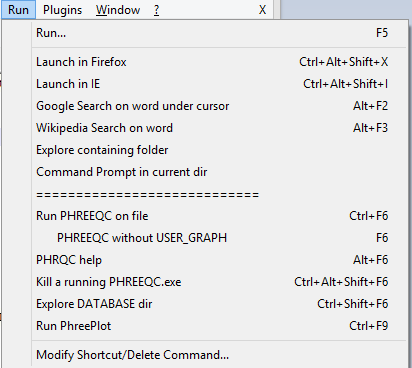
\includegraphics[width=100mm]{figures/notepad++run_menu.png}
\caption{PHREEQC software called from the Notepad++ Plugin}
\label{fig:phreeqc-notepad++3}
\end{figure}

\subsection{File formats}
All of the files discussed above are in the \emph{ASCII} text files format and, therefore, any regular text editor can be used. 
It is recommended that the editing of \emph{PHREEQC} files be done by using the NotPhreeqcce or notepad++ adapted version \cite{NotPhree:11}.

% IDEM - ACHO DESNECESSÁRIO
\subsection{Software Environment and Installation Procedures}
\emph{PHREEQC} has support for Windows (32 and 64-bit), MacOS (OS 10.6+) and Linux. \emph{PHREEQC} is currently on version 3 and with frequent updates, bug fixes and maintenance.

The \emph{PHREEQC} version for Windows has a self-extracting file that is available for download from the USGS website and easily installed. The \emph{UNIX} distribution comes with additional scripts and a makefile, and an instruction on how to compile and install the program.

%MINTEQ
\section{\emph{MINTEQ}}
\emph{MINTEQ} \cite{Felmy:84} is a geochemical program to model aqueous solutions and the interactions of aqueous solutions with hypothesized assemblages of solid phases. It has a particular inclination to calculate equilibrium composition of dilute aqueous solutions. The model is useful for calculating the equilibrium mass distribution among dissolved species, adsorbed species and multiple solid phases, although it has a much simpler treatment of the reactions. 

It was originally developed in FORTRAN77 by the \emph{Battelle Pacific Northwest Laboratory} (\emph{PNL}) and continues to be maintained by the \emph{Environmental Protection Agency} (\emph{EPA}) to perform the  necessary calculations regarding waste, sediments and ground water interaction. \emph{MINTEQ} does not consider the kinetic reactions and works at fixed temperature ($25$ degrees Celcius). 
An extensive database adequate to a broad range of problems is part of the software, and there is no need for the user to change nor add anything \cite{Brown:87} \cite{Allison:91}. The latest update on \emph{MINTEQ} dates from 1990, and since then, there has been only some improvements especially on the usability and calculations. This version was named \emph{MINTEQA2} and uses a well-developed thermodynamic database from the \emph{USGS}. During this review we will address the \emph{MINTEQA2} properties since it is the latest version and is clearly an improved version of the same program (\emph{MINTEQ}).

\subsection{Input/Output Options}
The input files for \emph{MINTEQA2} can be generated manually, but there is a supporting software called \emph{PRODEFA2} that guides the user to accomplish this task. \emph{PRODEFA2} is an interactive program used to create input files that will be addressed in details in section~\ref{minteq:interactions}. Four files compose the input of \emph{MINTEQA2}:
\begin{itemize}
\item Input file: The input file that contains the data input by the user. Typically, this file contains dissolved (i.e. Ca concentrations, pH, temperature) and solid phase (i.e. minerals, sorption sites) information for a water sample;
\item Database file: This file contains the thermodynamic constants that govern the processes of interest (i.e. complexation constants, mineral solubilities, activity constants) which will be used to conduct calculations;
\item Algorithm or executable file:  These files contain the algorithms of the code, which solve the specified problem (usually using an iterative numerical approach) within the constraints imposed by the Database files and the information in the Input file.
\item Output file: This file contains the results of the calculations performed by the Algorithm Files.
\end{itemize}

Among the input file's options, there are four levels of configuration. Each level controls some details of the simulation, and when these four levels are together, they compose a complete input file for \emph{MINTEQA2}. It is important to mention that if the user does not want to specify all the details, there are default options that enable any non-experienced user to execute simple simulations.
\begin{enumerate}
\item Displays the current settings of system parameters such as temperature as well as program flag settings such as the number of iterations allowed;
\item Specify the chemistry of the system;
\item This level works as a "line editor" in displaying by category or TYPE those species that have been explicitly entered through level 2;
\item Deals with utility functions (output file details, for example);
\end{enumerate}

If database, algorithm and output files are not specified, default options are used. Code ~\ref{minteqa2:input}  shows the \emph{MINTEQA2}'s input file used in the study case discussed in chapter~\ref{chapter:validation} and presented here as an example. The beginning of the file (first and second lines) contains a description of the simulation or input file; the third, fourth and fifth lines set configurations, such as temperature, unit chosen, eH, ionic strength, number of iterations, precipitation options. After that, the components that take part in the simulation, organized by internal id, concentration details and log of concentration are specified.

\begin{minipage}[c]{0.92\textwidth}
\begin{lstlisting}[frame=single, caption=\emph{MINTEQA2}'s input file, label=minteqa2:input]
LHDAMIANI - STUDY CASE
Comparative study           
25.00 MOLAL  0.000  0.00000E+00
0 0 1 0 1 0 0 0 1 1 0 0 0
0   0   0
    330  6.026E-09   -8.22 y                    /H+1               
    410  1.045E-02   -1.98 y                    /K+1               
    500  4.793E-01   -0.32 y                    /Na+1              
    150  1.053E-02   -1.98 y                    /Ca+2              
    460  5.439E-02   -1.26 y                    /Mg+2              
    732  2.889E-02   -1.54 y                    /SO4-2             
    180  5.595E-01   -0.25 y                    /Cl-1              

\end{lstlisting}
\end{minipage}



An excerpt of \emph{MINTEQA2}'s output is presented in Code ~\ref{minteqa2:output}, which shows important parameters of the solution's components. The whole output file is divided into six parts:
\begin{enumerate}
\item Reproduction and interpretation of the input file;
\item Detailed listing of species read from the database files;
\item Iteration information and detailed information for each species;
\item Percentage distribution of components among dissolved and adsorbed species;
\item Provisional or equilibrated mass distribution, provisional or equilibrium ionic strength, equilibrium pH and pE, electrostatic surface potential and charge for electrostatic adsorption models;
\item Saturation indices for all database solids with respect to the solution.
\end{enumerate}


\begin{minipage}[c]{0.92\textwidth}
\begin{lstlisting}[frame=single, caption=\emph{MINTEQA2}'s excerpt from the output file, label=minteqa2:output]
...
_______________________________________________________________________
______________________________ PART 3 of OUTPUT FILE __________________
  MINTEQA2  v4.02   DATE OF CALCULATIONS:  5-JUN-2000  TIME: 14: 6:27



PARAMETERS OF THE COMPONENT MOST OUT OF BALANCE:

ITER      NAME       TOTAL mol/L   DIFF FXN   LOG ACTVTY    RESIDUAL
0   SO4-2           1.580E-03   6.594E-07    -2.91757    5.014E-07
1   SO4-2           1.580E-03   4.193E-04    -2.91775    4.192E-04
2   SO4-2           1.580E-03   8.125E-06    -3.01997    7.967E-06
3   SO4-2           1.580E-03   1.693E-07    -3.02220    1.135E-08

 ID No  Name        Total Conc(M)    Conc (M)  log Activity   Diff fxn
  410   K+1            7.700E-05     7.649E-05    -4.14759    5.093E-11
  732   SO4-2          1.580E-03     1.266E-03    -3.02224    3.557E-09
    2   H2O            0.000E+00    -1.049E-05    -0.00004    0.000E+00
  330   H+1            0.000E+00     3.398E-03    -2.50000    0.000E+00
  140   CO3-2          0.000E+00     2.916E-17   -16.66004    0.000E+00

-----------------------------------------------------------------------
...
\end{lstlisting}
\end{minipage}

\subsection{User Interaction}\label{minteq:interactions}
\emph{MINTEQA2} and \emph{PRODEFA2} interactions are completely independent programs and \emph{PRODEFA2} is used before \emph{MINTEQA2} in order to generate the input file that will be consumed by the latter. Everything is done through the command prompt, as explained below. \emph{PRODEFA2} provides a "walk-through" to generate an input file for \emph{MINTEQA2}.

After starting the software and providing a valid name, it asks which part of the input file the user wants to create or edit (Figure~\ref{minteq:init}). We will follow the suggested order and go through 4 levels, as previously discussed in this section. Figure~\ref{minteq:level0} presents the main menu, which shows the organization of all the levels, and works as a central hub of information. Figure ~\ref{minteq:level1} displays the necessary information about level 1. To change any of the entries on this screen, the user must enter the number to the left of the entry and respond to the questions presented. All four levels are based on this type of interaction. Through these interactions, the user has access to the information in the database and can choose the data to be used for the model.

\begin{figure}[ht!]
\centering
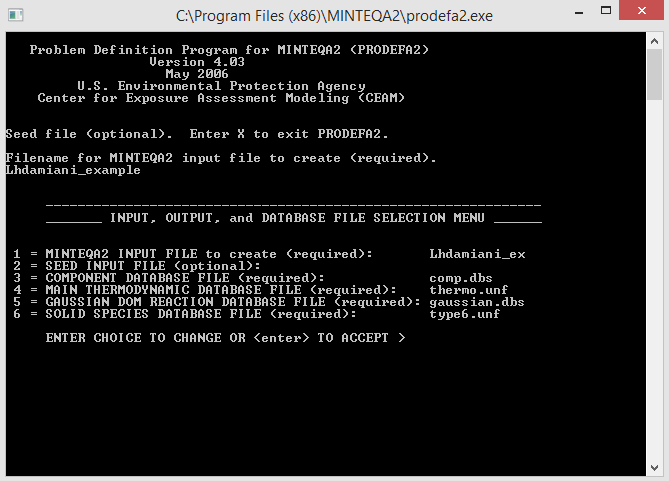
\includegraphics[width=100mm]{figures/minteq-init.png}
\caption{\emph{MINTEQA2} initial menu options}
\label{minteq:init}
\end{figure}

\begin{figure}[ht!]
\centering
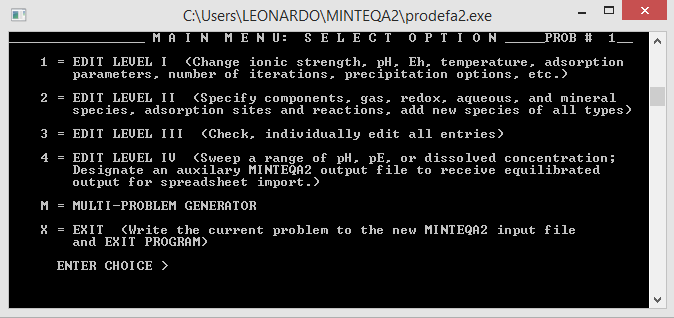
\includegraphics[width=100mm]{figures/minteq-level0.png}
\caption{\emph{MINTEQA2} main menu}
\label{minteq:level0}
\end{figure}

\begin{figure}[ht!]
\centering
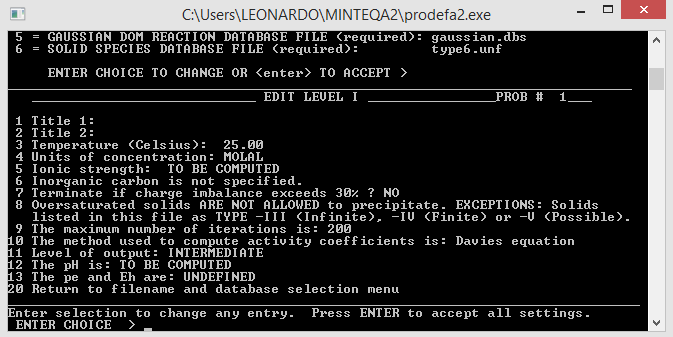
\includegraphics[width=100mm]{figures/minteq-level1.png}
\caption{\emph{MINTEQA2} Level 1 information}
\label{minteq:level1}
\end{figure}


For example, we chose to add a specific aqueous species to show the \emph{PRODEFA2} interactions and present it step-by-step bellow:

\begin{enumerate}
\item Choose level 2 on main menu;
\item Choose option 1 (Specify AQUEOUS COMPONENTS: TOTAL CONCENTRATIONS or FIXED ACTIVITIES) inside the menu from level 2;
\item Choose option 1 (TOTAL DISSOLVED CONCENTRATION), it identifies how we want to entre this new component.
\item At this step, we are requested to enter the first letter for the component. Alternatives to this approach is to enter "-1" if you know the component id number or quit. We will add \ce{Na^+} to the system, and type the letter "N" and hit the enter button.
\item At this step, all the existing options available are shown. listed with an identifier. We are also requested to identify one of these to be added. This can be seen in ~\ref{minteq:Na+}.
\item After pressing \ce{Na^+}'s id (at this case was the number 4). We can finally enter the TOTAL DISSOLVED CONCENTRATION (MOLAL) of COMPONENT defined earlier on step 3. After adding the molal concentration for this species the system goes back to step 4 in case we want to continue adding other components.
\end{enumerate}

\begin{figure}[ht!]
\centering
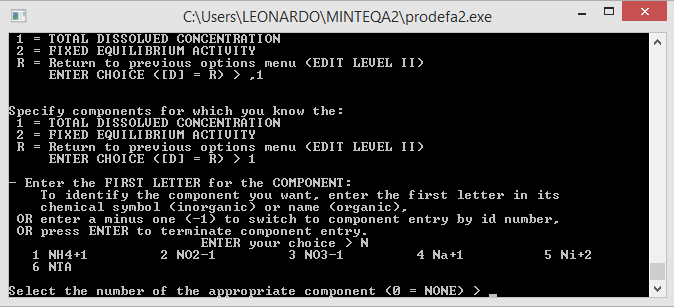
\includegraphics[width=100mm]{figures/minteq-Na+.png}
\caption{\emph{PRODEFA2}'s example of adding a specific aquoues species (\ce{Na+}) }
\label{minteq:Na+}
\end{figure}

There is also a software called \emph{Visual Minteq} that tries to "humanize" \emph{MINTEQ} and was maintained by the KTH Royal Institute of Technology (Stockholm, Sweden). The latest release  (version 3.0) of \emph{Visual Minteq} dates back to December 2013, and it is available only for \emph{Windows} operating systems, since it was developed in Visual Basic. 

\subsection{File formats}
All the files follow a regular text format (\emph{ASCII}) and their purpose is defined in the extension of the file. 
\begin{itemize}
\item Input files have the extension \emph{"INP"};
\item Test and help files have the extension \emph{"HLP"};
\item Output files have the extension \emph{"LST"};
\item Database files have the extension \emph{"DBS"} or \emph{"UNF"};
\item Input file have the extension \emph{"INP"};
\end{itemize}


% Juntei as duas partes como tu sugeriu.. deixei a parte de installation procedures .. qualquer coisa posso tirar depois se decidirmos nao utilizar.
\subsection{Software Environment and Installation Procedures}
\emph{MINTEQA2} is currently at the version 4.03 (Windows only), and this release dates back to May 2006. The latest \emph{UNIX} distribution is version 3.12 (which was also called BETA for UNIX) and dates back to August 1996.
\emph{MINTEQA2} is easily installed by a self-extractor installer that can be downloaded from \emph{EPA}'s website \cite{minteq:website} and \cite{minteq:unix}. Included in the distribution package are also some important documentation, \emph{PRODEFA2} software and several input/output template files.
The UNIX version distribution comes with the source files and must be compiled and linked to run.

\section{\emph{SOLMINEQ.88}}
\emph{SOLMINEQ.88}  is a geochemical modeling program written in FORTRAN77 and based on SOLMNEQ \cite{Kharaka:73} with improved algorithms that resulted in a faster program execution and tighter convergence. The software has a database with the focus on organics aqueous species. It calculates the distribution of mass among aqueous species and complexes, and calculates saturation indices of minerals at different temperatures and pressures. It includes options as boiling, mixing of solutions, and partitioning of gases between water, oil and vapor phases. \emph{SOLMINEQ.88} also provides for mass transfer with the effects of dissolution and precipitation of minerals and options to calculate activity coefficients \cite{Kharaka:88}. The original version has no UI, but there were further studies with the intention of creating a user-friendly program that can be used to generate, edit and analyze input and output files - \emph{SOLINPUT}.
\emph{SOLMINEQ.88} model has not been developed any further nor improved since its first release.

\subsection{Input/Output Options}
The input of \emph{SOLMINEQ.88} consists of two sets of data: fixed and variable. The first data contains the chemical composition of an aqueous fluid and options for processing these data; and the second data consists of the input required for using the first set of data.

The input file consists of six parts, and \emph{SOLINPUT} guides the user through all of them:
\begin{enumerate}
\item Basic Parameters: enter the chemical and physical data for that sample;
\item Flags: controls how the software interprets, processes, and displays the data;
\item pH: controls the details of how the pH calculation is done;
\item Mass transfer: defines which mass transfer capabilities are used;
\item User Log K: makes temporary changes and extensions to the database;
\item Additional ions and minerals: temporarily adds user defined ions and minerals to a particular simulation;
\end{enumerate}

The output file contains the results produced by \emph{SOLMINEQ.88}, and also consists of six parts: 
\begin{enumerate}
\item An input data echo that shows the values and options selected for each sample; 
\item A table listing the calculated tolerance factor for successive iterations on the anions; 
\item A list of input to \emph{SOLMINEQ.88} including sample description, pH, Eh, temperature and so on; 
\item A table showing the distribution of species in solution; 
\item Ratios of a number of important cations and anions ; and 
\item A table indicating the states of reactions for minerals considered.

\begin{minipage}[c]{0.92\textwidth}
\begin{lstlisting}[frame=single, caption=\emph{SOLMINEQ.88}'s excerpt from the output file, label=solmineq:output]
 : Test Sample #1 for SOLMINEQ.88 - Modified Seawater at 25 C
TEMP HI TEMP DENS PRESS
0.2500E+02 O.OOOOE+00 0.1023E+01 O.OOOOE+00
PH EHM EHMC EMFZSC
0.8200E+01 0.5000E+00 0.9000E+01 0.9000E+01
CONCENTRATION UNITS : PPM
Na K Li Ca
0.1077E+05 0.3991E+03 0.1810E+00 0.4123E+03
Si02 Cl S04 H2S
0.4280E+01 0.1935E+05 0.2712E+04 O.OOOOE+00
F P04 N03 NH3
0.1390E+01 0.6000E-01 0.2900E+00 0.3000E-01
Pb Zn Cu Mn
0.5000E-04 0.4900E-02 0.7000E-03 0.2000E-03
As U V
0.4000E-02 O.OOOOE+00 O.OOOOE+00
Acetate Oxalate Succinate CH4
0.1000E+00 0.1000E+00 0.1000E+00 0.1000E+00
\end{lstlisting}
\end{minipage}

\subsection{User Interaction}
The software that accompanies \emph{SOLMINEQ.88} and handles the generation of input files and all the interactions is named \emph{SOLINPUT} and described in \cite{Debraal:89}. All interactions are through command prompt input following displayed menus with several options. The user selects the option by entering the indication number and pressing enter (the indication number stays on the left of the option). Figure~\ref{solmineq:interaction} shows this example of interaction.

\begin{minipage}[c]{0.92\textwidth}
\begin{lstlisting}[frame=single, caption=\emph{SOLMINEQ.88}'s example of user interaction, label=solmineq:interaction]
	pH OPTIONS
1) Gas Addition Option
2) Gas-Water-Oil Distribution Option
3) Carbonate Mineral Saturation Option
4) C02 Option
5) Tolerance factor for Mineral and C02 Options
6) Return to Options Menu
Enter Choice (1-6)   __
\end{lstlisting}
\end{minipage}

\subsection{File formats}
All the files that \emph{SOLMINEQ.88} deals are regular \emph{ASCII} text files and any text editor can be used to create, edit or view the files. The database files from \emph{SOLMINEQ.88} have the extension "TBL", while the input and output files, "IN" and "OUT", respectively. 
Some optional file with the extension "MIXFLE" can be used to specify mixture properties. Finally, if the user activates the restart option, also known as pickup option, the file "OUTIN" will be generated and it contains data from the current run.

\subsection{Software Environment and Installation Procedures}
As mentioned, \emph{SOLMINEQ.88} had only one release and has been discontinued since then. It is available only for the \emph{Windows} operating system.

\emph{SOLMINEQ.88} distribution requires knowledge of compiling and linking \emph{FORTRAN77} programs. It also comes with the software \emph{SOLINPUT}.

\section{Existing Thermodynamic datasets}
The contents of the databases are extracted from the \emph{Lawrence Livermore National Laboratory (LLNL)} thermodynamic datasets that are used in \emph{EQ3/6}, \emph{PHREEQC} and others. The data sets are contributions from many authors that had measured thermodynamical and kinetic parameters of the minerals and reactions minerals over the years. Interaction with flat file databases are difficult and, if necessary, must be done carefully - the format of the file is composed of a series of rules and very often is not recommended that the user alters anything inside the flat file database due to the complexity and the errors that it might result. The following is a small excerpt that illustrates the structure of information in the \emph{LLNL}'s flat file:

\begin{itemize}
\item Parameters: Many used parameters are stablished on this section, among them are temperatures, pressures, debye huckel coefficients, bdot coefficients...
\begin{lstlisting}[frame=single, caption=Excerpt of the section Parameters]
* temperatures
         0.0000   25.0000   60.0000  100.0000
       150.0000  200.0000  2500000  300.0000
* pressures
         1.0134    1.0134    1.0134    1.0134
         4.7600   15.5490   39.7760   85.9270
\end{lstlisting}
\item Elements: This section is composed of information on pure elements. It also lists the mole weights of elements and the abreviation: 
\begin{lstlisting}[frame=single, caption=Excerpt of the section Elements]
Oxygen          (O )          mole wt.=   15.9994
Silver          (Ag)          mole wt.=  107.8680
Aluminum        (Al)          mole wt.=   26.9815
\end{lstlisting}
\item Basic Species: This section lists atomic or molecular structural units for a mineral:
\begin{lstlisting}[frame=single, caption=Excerpt of the section Basic Species]
H2O
     charge=  0.0      ion size=  0.0 A      mole wt.=   18.0152
     2 elements in species
       1.000 O               2.000 H
\end{lstlisting}


\item Redox Couples: This sections includes all chemical reactions in which molecules have their oxidation states changed. 
Redox reactions involve the transfer of electrons between species.
The name comes from two concepts involved with electron transfer (reduction - loss of electrons - and oxidation - gain of electrons). Example:

\begin{minipage}[c]{0.92\textwidth}
\begin{lstlisting}[frame=single, caption=Excerpt of the section Redox Couples]
Cr++
     charge=  2.0      ion size=  5.0 A      mole wt.=   51.9960 g
     4 species in reaction
      -1.000 H+              0.500 H2O             1.000 Cr+++
      -0.250 O2(aq)
        33.6814   29.9291   25.6126   21.6721
        17.7896   14.7267   12.2289   10.1676
\end{lstlisting}
\end{minipage}


\item Aqueous Species: This sections contains the water solutions. The word aqueous is applied to a solution or mixture in which water is the solvent. When a chemical species has been dissolved in water, this is denoted by writing (aq) after the chemical name. Example:

\begin{minipage}[c]{0.92\textwidth}
\begin{lstlisting}[frame=single, caption=Excerpt of the section Aqueous Species]
CO2(aq)
     charge=  0.0      ion size=  4.0 A      mole wt.=   44.0098 g
     3 species in reaction
      -1.000 H2O             1.000 H+              1.000 HCO3-
        -6.5570   -6.3660   -6.3325   -6.4330
        -6.7420   -7.1880   -7.7630   -8.4650
\end{lstlisting}
\end{minipage}

\item Minerals: This sections lists the physical properties and chemical formula of minerals: 

\begin{minipage}[c]{0.92\textwidth}
\begin{lstlisting}[frame=single, caption=Excerpt of the section Minerals]
Calcite                         type= carbonate
     formula= CaCO3
     mole vol.=   36.934 cc      mole wt.=  100.0892 g
     3 species in reaction
       1.000 Ca++            1.000 HCO3-          -1.000 H+
         2.0683    1.7130    1.2133    0.6871
         0.0762   -0.5349   -1.2301   -2.2107
\end{lstlisting}
\end{minipage}

\item Gases: This section lists individual atoms (e.g. noble gases or atomic gases), elemental molecules made from one type of atom (e.g. oxygen), or compounds made up of two or more molecules (e.g. carbon dioxide). Example: 

\begin{minipage}[c]{0.92\textwidth}
\begin{lstlisting}[frame=single, caption=Excerpt of the section Gases]
CO2(g)
     mole wt.=   44.0098 g
     3 species in reaction
      -1.000 H2O             1.000 H+              1.000 HCO3-
        -7.6827   -7.8184   -8.0628   -8.3849
        -8.8297   -9.3208   -9.8841  -10.6132
\end{lstlisting}
\end{minipage}

\item Oxides: This sections contains the chemical compounds that consists of at least one oxygen atom and one other element in its chemical formula, and also does not include silica (Si): 

\begin{minipage}[c]{0.92\textwidth}
\begin{lstlisting}[frame=single, caption=Excerpt of the section Oxides]
Al2O3
     mole wt.=  101.9616 g
     3 species in reaction
      -6.000 H+              2.000 Al+++           3.000 H2O
\end{lstlisting}
\end{minipage}
\end{itemize}

%GEOCHEMICAL SPECIATION ANALYSIS
\section{Discussion}
In this section some important aspects and issues of each software presented earlier are compared and discussed. 


From a computational point of view, we analysed and evaluated the software engineering aspects of current solutions.  The following aspects were taken into consideration:
\begin{itemize}
\item Costs: Costs are probably the most important thing that people look first when choosing software. However, it should not be the deciding factor. Different solutions use different pricing models, according to the purpose and utilization of the software.

\item Setup and versioning: The installation of software is the act of making it ready for execution. Depending on the software different options are used to copy/generate files from the installation files to the local computer to be accessed by the operating system (OS). The OS also influences how this process is done. Each software has a different distribution package for different OS. Commonly software are distributed only to specific OS. Also common are software with disparate versions according to the OS, resulting in divergent features available on the same software defined by the OS types.

\item Customization and Integration: Is the software a standard solution, and its supplier interested in making changes? This is the typical scenario where the user has high probability of finding problems ahead. Therefore, an interesting exercise is to think of how this software communicates with others. Options like  ``import'' and ``export'' are vital when working with a large amount of data, allowing different tools to be used to analyse the output, with the purpose of reaching deeper insights from the information available. 

\item Security and Control: Security is one of the main issues one faces when considering a software. Data privacy is an important criteria. Ensuring that the software can guarantee no data loss or data leakage is important. The solutions that provide direct control to the database, details, and processes are most likely to require data privacy.

\item Infrastructure: When choosing a software, the infrastructure it requires need to be carefully analyzed. Does it require Internet access? How much space on disk and memory does it use? Extra costs may be incurred if this is not addressed.

\item Core functionality: This is one of the most important points to be analyzed. How good is the software focus on the needs of the user, and how good is the value the software brings to its users?

\item Graphical User Interface (\emph{GUI}) and visualization: This feature handles the interaction between the users and the software. When the software is within a complex domain, such as geochemical modeling, the \emph{GUI} is even more important. It is responsible for allowing the user to consider all necessary possible options. 

\item Support and Maintenance: If the software, for some unknown reason, goes down, is the user able to reach someone for troubleshooting? Will the user be able to find a users' community to debate and share knowledge? If the software has a support team working to fix bugs, improve the performance, add new features and sharpen some of the old features, it means that the user will have a better infrastructure to work with.

\item Database: All the data manipulated inside a software is stored and organized in a database. There are multiple ways of doing this. Many important things must be taken into account to decide which database fits best to the software. Since the 80's the relational database model has been the most popular. A conceptual database model is strongly recommended to produce a schema that considers all the structure and information needed by this software. Along the database schema, the security of this database must be addressed properly, for consistency and privacy. A good database design avoids redundant data (unnecessarily duplicated data). Poorly designed database generates inconsistent data (inaccurate data), which will lead to wrong decisions and, therefore, can result in failure of the software. We have observed that current solutions are mostly based on text input and output files, without a proper database. 
\end{itemize}


To achieve an applicable comparison, we give grades from 1 to 5 to each aspect (where 1 is the lowest and 5 the highest possible grade). This "grading system" is done with the intention of comparing and normalizing the attributes of the software (see table ~\ref{tab:comparativeSoftwareTable}\footnote{Source:Author}).

\begin{table}
\caption{Qualitative analysis of the Geochemical Speciation Software}
\label{tab:comparativeSoftwareTable}
\centering
\begin{tabular}{r|ccccccccc|ccc}

SOFTWARE &
\rot{Costs} &
\rot{Setup and versioning} & 
\rot{Customization and Integration} &
\rot{Security and Control} &
\rot{Infrastructure} &
\rot{Core functionality} &
\rot{Graphical User Interface} &
\rot{Support and Maintenance} &
\rot{Database}  &
\rot{Overall Average} 
    \\ \hline
EQ3/6        	& 2 & 2 & 1 & 1 & 3 & 5 & 1 & 1 & 1 & 1.88 \\ 
PHREEQC         & 4 & 4 & 2 & 2 & 3 & 4 & 2 & 3 & 1 & 2.77 \\ 
MINTEQA2        & 4 & 2 & 1 & 1 & 2 & 2 & 1 & 1 & 1 & 1.66\\ 
SOLMINEQ.88	    & 3 & 1 & 1 & 1 & 1 & 5 & 1 & 1 & 1 & 1.66\\ 
\hline
\end{tabular}
\end{table}





\newpage

%SUMMARY
\section{Summary}

Regarding geochemical features, Table~\ref{tab:comparativeTable} shows characteristics and features of the different software solutions.

\begin{table}
\caption{Geochemical comparison between the different speciation software}
\label{tab:comparativeTable}
\centering
\begin{tabular}{r|cccccccc}
SOFTWARE &
\rot{Aqueous Complexation} &
\rot{Precipitation and Dissolution Mass Balancing} & 
\rot{Reaction path} &
\rot{Kinetics} &
\rot{Multi-Activity Coefficient methods} 
    \\ \hline
EQ3/6        	&  \OK &  \OK & \OK & \OK & \OK    \\ 
PHREEQC        &  \OK &  \OK  & \OK & \OK &  \\
MINTEQA2        &  \OK  &  \OK & & &    \\ 
SOLMINEQ.88	& \OK& \OK&\OK & \OK & \OK\\
\hline
\end{tabular}
\end{table}


\begin{itemize}
\item EQ3/6: It represents a landmark in Geochemical Modeling. Unfortunately, it is inaccessible due to the elevated cost of licensing. The vast amount of information available online about \emph{EQ3/6} makes it an excellent source of information.  It used the computing tools and options that were available in 1970’s and 80’s, until the latest known release date in 1992. Since then, computing has clearly evolved, making it an obsolete and difficult to use. It has a large database with many pieces of information, but the contents are not transparent. It is hard to understand what exactly is the software doing; verifying if that is what the users wants is even more difficult. It is also important to mention that in \emph{EQ3/6}  documentation it recommends the user to use operating system commands (i.e. \emph{ctrl+c}) to interact with the software - which is a highly risky procedure in modern computers.

\item PHREEQC: It is the best option for users not experienced with software. It has a \emph{GUI} and comes with a self-extractor installer. Important to mention here is that \emph{PHREEQC}'s \emph{GUI} is far from what a typical user of current era might expect. It is not clear in many aspects, and its usability is far from regular. In the geochemical modeling area, not all the users are familiar with tasks as compiling and linking computer programs. \emph{PHREEQC} allows anyone with an interest to have a chance to perform a geochemical modeling simulation, even as many people have different ways of defining the problem. Database in \emph{PHREEQC} seems to be a problem, as it uses a flat file database.

\item MINTEQA2: From the geochemical point of view, \emph{MINTEQA2} is the simpler of the four software analyzed in this work. The user interaction can be painful for anyone who are not familiar with command prompts. The complexity of the input file also makes it difficult to use. Creating an input file without the subsidiary software \emph{PRODEFA2} is a task close to impossible and learning how to use this subsidiary software is a very costly task. Taking into account that its last release dates back to 2006, it is difficult to justify using \emph{MINTEQA2}.

\item SOLMINEQ.88: This is another software that was a pioneer and laid the groundwork for many others to improve and progress the knowledge of geochemical modeling. \emph{SOLMINEQ} used the computing tools that were accessible when it was developed in 1980’s. There are less costly options easily attainable today, thus it is no longer a popular option for geochemical modeling.


\end{itemize}